\newcommand{\comp}{\TT{comp()}\xspace}
\chapter{Указатели на функции}
\label{sec:pointerstofunctions}

\myindex{\CLanguageElements!\Pointers}
Указатель на функцию, в целом, как и любой другой указатель, просто адрес, указывающий на начало функции 
в сегменте кода.

\myindex{Callbacks}
Это часто применяется для вызовов т.н. callback-функций \footnote{\href{http://go.yurichev.com/17071}{wikipedia}}.

Известные примеры:

\begin{itemize}
\item \qsort\footnote{\href{http://go.yurichev.com/17072}{wikipedia}},
{\TT{atexit()}}\footnote{\url{http://go.yurichev.com/17073}} из стандартной библиотеки Си; 

\item сигналы в *NIX ОС\footnote{\href{http://go.yurichev.com/17074}{wikipedia}};

\item запуск тредов: \TT{CreateThread()} (win32), \TT{pthread\_create()} (POSIX);

\item множество функций win32, например \TT{EnumChildWindows()}\footnote{\href{http://go.yurichev.com/17075}{MSDN}}.

\item множество мест в ядре Linux, например, функции драйверов файловой системы вызываются
через callback-и: 
\url{http://go.yurichev.com/17076}

\item функции плагинов GCC также вызываются через callback-и: 
\url{http://go.yurichev.com/17077}

\item Один из примеров указателей на функции это таблица в оконном менеджере \q{dwm} для Linux, описывающая шорт-каты.

Каждый шорт-кат имеет соответствующую функцию, которую нужно вызвать, если эта клавиша нажата: \href{http://go.yurichev.com/17078}{GitHub}.
Как мы видим, с такой таблицей намного легче обходится чем с большим выражением switch().

\end{itemize}

\myindex{\CStandardLibrary!qsort()}
Итак, функция \qsort это реализация алгоритма \q{быстрой сортировки}. 
Функция может сортировать что угодно, 
любые типы данных, но при условии, что вы имеете функцию сравнения этих двух элементов данных и 
\qsort может вызывать её.

Эта функция сравнения может определяться так:

\begin{lstlisting}
int (*compare)(const void *, const void *)
\end{lstlisting}

Воспользуемся немного модифицированным примером, который был найден \href{http://go.yurichev.com/17079}{здесь}:

\lstinputlisting[numbers=left,label=qsort_c_src]{patterns/18_pointers_to_functions/17_1.c}

\section{MSVC}

Компилируем в MSVC 2010 (некоторые части убраны для краткости) с опцией \TT{\Ox}:

\lstinputlisting[caption=\Optimizing MSVC 2010: /GS- /MD]{patterns/18_pointers_to_functions/17_2_msvc_Ox.asm}

Ничего особо удивительного здесь мы не видим. В качестве четвертого аргумента, 
в \qsort просто передается адрес метки \TT{\_comp}, где собственно и располагается функция \comp,
или, можно сказать, самая первая инструкция этой функции.

Как \qsort вызывает её?

\myindex{Windows!MSVCR80.DLL}
Посмотрим в MSVCR80.DLL (эта DLL куда в MSVC вынесены функции из стандартных библиотек Си):

\lstinputlisting[caption=MSVCR80.DLL]{patterns/18_pointers_to_functions/17_3_MSVCR.lst}

\TT{comp} --- это четвертый аргумент функции. 
Здесь просто передается управление по адресу, указанному в \TT{comp}. 
Перед этим подготавливается два аргумента для функции \comp. 
Далее, проверяется результат её выполнения.

Вот почему использование указателей на функции ~--- это опасно. 
Во-первых, если вызвать \qsort с неправильным указателем на функцию, 
то \qsort, дойдя до этого вызова, может передать управление неизвестно куда, 
процесс упадет, и эту ошибку можно будет найти не сразу.

Во-вторых, типизация callback-функции должна строго соблюдаться, 
вызов не той функции с не теми аргументами не того типа, 
может привести к плачевным результатам, 
хотя падение процесса это и не проблема, проблема ~--- это найти ошибку, ведь компилятор 
на стадии компиляции может вас и не предупредить о потенциальных неприятностях.

\clearpage
\subsectionold{MSVC + \olly}
\myindex{\olly}

Загрузим наш пример в \olly и установим точку останова на функции \comp{}.
Как значения сравниваются, мы можем увидеть во время самого первого вызова \comp{}:

\begin{figure}[H]
\centering
\myincludegraphics{patterns/18_pointers_to_functions/olly1.png}
\caption{\olly: первый вызов \comp}
\label{fig:qsort_olly1}
\end{figure}

Для удобства, \olly показывает сравниваемые значения в окне под окном кода.
Мы можем так же увидеть, что \ac{SP} указывает на \ac{RA} где находится место в функции \qsort (на самом деле, находится в \TT{MSVCR100.DLL}).

\clearpage
Трассируя (F8) до инструкции \TT{RETN} и нажав F8 еще один раз, мы возвращаемся в функцию \qsort:

\begin{figure}[H]
\centering
\myincludegraphics{patterns/18_pointers_to_functions/olly2.png}
\caption{\olly: код в \qsort сразу после вызова \comp}
\label{fig:qsort_olly2}
\end{figure}

Это был вызов функции сравнения.

\clearpage
Вот также скриншот момента второго вызова функции \comp{}---теперь сравниваемые значения другие:

\begin{figure}[H]
\centering
\myincludegraphics{patterns/18_pointers_to_functions/olly3.png}
\caption{\olly: второй вызов \comp}
\label{fig:qsort_olly3}
\end{figure}


\subsection{MSVC + tracer}
\myindex{tracer}

Посмотрим, какие пары сравниваются.
Эти 10 чисел будут сортироваться: 
1892, 45, 200, -98, 4087, 5, -12345, 1087, 88, -100000.

Найдем адрес первой инструкции \CMP в \comp и это \TT{0x0040100C} и мы ставим точку останова на ней:%

\begin{lstlisting}
tracer.exe -l:17_1.exe bpx=17_1.exe!0x0040100C
\end{lstlisting}

Получаем информацию о регистрах на точке останова:

\begin{lstlisting}
PID=4336|New process 17_1.exe
(0) 17_1.exe!0x40100c
EAX=0x00000764 EBX=0x0051f7c8 ECX=0x00000005 EDX=0x00000000
ESI=0x0051f7d8 EDI=0x0051f7b4 EBP=0x0051f794 ESP=0x0051f67c
EIP=0x0028100c
FLAGS=IF
(0) 17_1.exe!0x40100c
EAX=0x00000005 EBX=0x0051f7c8 ECX=0xfffe7960 EDX=0x00000000
ESI=0x0051f7d8 EDI=0x0051f7b4 EBP=0x0051f794 ESP=0x0051f67c
EIP=0x0028100c
FLAGS=PF ZF IF
(0) 17_1.exe!0x40100c
EAX=0x00000764 EBX=0x0051f7c8 ECX=0x00000005 EDX=0x00000000
ESI=0x0051f7d8 EDI=0x0051f7b4 EBP=0x0051f794 ESP=0x0051f67c
EIP=0x0028100c
FLAGS=CF PF ZF IF
...
\end{lstlisting}

Отфильтруем \TT{EAX} и \TT{ECX} и получим:

\begin{lstlisting}
EAX=0x00000764 ECX=0x00000005
EAX=0x00000005 ECX=0xfffe7960
EAX=0x00000764 ECX=0x00000005
EAX=0x0000002d ECX=0x00000005
EAX=0x00000058 ECX=0x00000005
EAX=0x0000043f ECX=0x00000005
EAX=0xffffcfc7 ECX=0x00000005
EAX=0x000000c8 ECX=0x00000005
EAX=0xffffff9e ECX=0x00000005
EAX=0x00000ff7 ECX=0x00000005
EAX=0x00000ff7 ECX=0x00000005
EAX=0xffffff9e ECX=0x00000005
EAX=0xffffff9e ECX=0x00000005
EAX=0xffffcfc7 ECX=0xfffe7960
EAX=0x00000005 ECX=0xffffcfc7
EAX=0xffffff9e ECX=0x00000005
EAX=0xffffcfc7 ECX=0xfffe7960
EAX=0xffffff9e ECX=0xffffcfc7
EAX=0xffffcfc7 ECX=0xfffe7960
EAX=0x000000c8 ECX=0x00000ff7
EAX=0x0000002d ECX=0x00000ff7
EAX=0x0000043f ECX=0x00000ff7
EAX=0x00000058 ECX=0x00000ff7
EAX=0x00000764 ECX=0x00000ff7
EAX=0x000000c8 ECX=0x00000764
EAX=0x0000002d ECX=0x00000764
EAX=0x0000043f ECX=0x00000764
EAX=0x00000058 ECX=0x00000764
EAX=0x000000c8 ECX=0x00000058
EAX=0x0000002d ECX=0x000000c8
EAX=0x0000043f ECX=0x000000c8
EAX=0x000000c8 ECX=0x00000058
EAX=0x0000002d ECX=0x000000c8
EAX=0x0000002d ECX=0x00000058
\end{lstlisting}

Это 34 пары.
Следовательно, алгоритму быстрой сортировки нужно 34 операции сравнения для сортировки этих 10-и чисел.

\clearpage
\subsection{MSVC + tracer (code coverage)}
\myindex{tracer}

Но можно также и воспользоваться возможностью tracer накапливать все возможные состояния регистров и показать их в \IDA.

Трассируем все инструкции в функции \comp:

\begin{lstlisting}
tracer.exe -l:17_1.exe bpf=17_1.exe!0x00401000,trace:cc
\end{lstlisting}

Получем .idc-скрипт для загрузки в \IDA и загружаем его:

\begin{figure}[H]
\centering
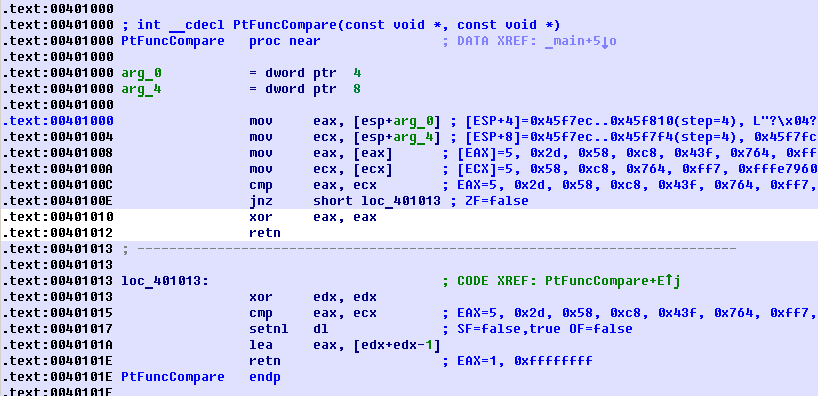
\includegraphics[scale=\FigScale]{patterns/18_pointers_to_functions/tracer_cc.png}
\caption{tracer и IDA. N.B.: 
некоторые значения обрезаны справа}
\label{fig:qsort_tracer_cc}
\end{figure}

Имя этой функции (PtFuncCompare) дала \IDA --- видимо, потому что видит что указатель на эту функцию передается в \qsort.

Мы видим, что указатели $a$ и $b$ указывают на разные места внутри массива, 
но шаг между указателями --- 4, что логично, ведь в массиве хранятся 32-битные значения.

Видно, что инструкции по адресам \TT{0x401010} и \TT{0x401012} никогда не исполнялись (они и остались белыми): 
действительно, функция \comp никогда не возвращала 0,
потому что в массиве нет одинаковых элементов.

\section{GCC}

Не слишком большая разница:

\begin{lstlisting}[caption=GCC]
                lea     eax, [esp+40h+var_28]
                mov     [esp+40h+var_40], eax
                mov     [esp+40h+var_28], 764h
                mov     [esp+40h+var_24], 2Dh
                mov     [esp+40h+var_20], 0C8h
                mov     [esp+40h+var_1C], 0FFFFFF9Eh
                mov     [esp+40h+var_18], 0FF7h
                mov     [esp+40h+var_14], 5
                mov     [esp+40h+var_10], 0FFFFCFC7h
                mov     [esp+40h+var_C], 43Fh
                mov     [esp+40h+var_8], 58h
                mov     [esp+40h+var_4], 0FFFE7960h
                mov     [esp+40h+var_34], offset comp
                mov     [esp+40h+var_38], 4
                mov     [esp+40h+var_3C], 0Ah
                call    _qsort
\end{lstlisting}

Функция \comp:

\begin{lstlisting}
                public comp
comp            proc near

arg_0           = dword ptr  8
arg_4           = dword ptr  0Ch

                push    ebp
                mov     ebp, esp
                mov     eax, [ebp+arg_4]
                mov     ecx, [ebp+arg_0]
                mov     edx, [eax]
                xor     eax, eax
                cmp     [ecx], edx
                jnz     short loc_8048458
                pop     ebp
                retn
loc_8048458:
                setnl   al
                movzx   eax, al
                lea     eax, [eax+eax-1]
                pop     ebp
                retn
comp            endp
\end{lstlisting}

\myindex{Linux!libc.so.6}
Реализация \qsort находится в \TT{libc.so.6}, и представляет собой просто wrapper
\footnote{понятие близкое к \gls{thunk function}} для \TT{qsort\_r()}.

Она, в свою очередь, вызывает \TT{quicksort()}, где есть вызовы определенной нами функции через переданный указатель:


\begin{lstlisting}[caption=
(файл libc.so.6{,} версия glibc\EMDASH{}2.10.1)]

.text:0002DDF6                 mov     edx, [ebp+arg_10]
.text:0002DDF9                 mov     [esp+4], esi
.text:0002DDFD                 mov     [esp], edi
.text:0002DE00                 mov     [esp+8], edx
.text:0002DE04                 call    [ebp+arg_C]
...
\end{lstlisting}

\subsection{GCC + GDB (с исходными кодами)}
\myindex{GDB}

Очевидно, у нас есть исходный код нашего примера на Си (\myref{qsort_c_src}), 
так что мы можем установить точку останова ($b$) на номере строки
(11-й --- это номер строки где происходит первое сравнение).
Нам также нужно скомпилировать наш пример с ключом \TT{-g}, чтобы в исполняемом файле была
полная отладочная информация.
Мы можем так же выводить значения используя имена переменных (\TT{p}):
отладочная информация также содержит информацию о том, в каком регистре и/или элементе локального
стека находится какая переменная.

\myindex{Glibc}
Мы можем также увидеть стек (\TT{bt}) и обнаружить что в Glibc используется какая-то вспомогательная функция с именем
 
\TT{msort\_with\_tmp()}.

\lstinputlisting[caption=GDB-сессия]{patterns/18_pointers_to_functions/GDB_source.txt}

\subsection{GCC + GDB (без исходных кодов)}
\myindex{GDB}

Но часто никаких исходных кодов нет вообще, так что мы можем дизассемблировать функцию \comp (\TT{disas}), 
найти самую первую инструкцию \CMP и установить точку останова ($b$) по этому адресу.
На каждой точке останова мы будем видеть содержимое регистров (\TT{info registers}).
Информация из стека так же доступна (\TT{bt}), 
но частичная: здесь нет номеров строк для функции \comp.

\lstinputlisting[caption=GDB-сессия]{patterns/18_pointers_to_functions/GDB_no_source.txt}

